\section{GloVe – Global Vectors}
\begin{frame}{}
    \LARGE GloVe – Global Vectors
\end{frame}

\begin{frame}[allowframebreaks]{GloVe – Global Vectors}
    \textbf{Proposed by:} Pennington et al., 2014

    \begin{itemize}
        \setlength{\itemsep}{1em}
        \item Combines global matrix factorization with local context windows.
        \item Captures co-occurrence statistics of words across entire corpus.
        \item Embeddings reflect ratios of co-occurrence probabilities.
    \end{itemize}

\framebreak
    \textbf{Loss function:}
    \[
        J = \sum_{i,j=1}^{V} f(X_{ij}) \left( w_i^\top \tilde{w}_j + b_i + \tilde{b}_j - \log X_{ij} \right)^2
    \]
    where:
    \begin{itemize}
        \setlength{\itemsep}{1em}
        \item $X_{ij}$: number of times word $j$ occurs in the context of word $i$
        \item $P_{ij}$: probability of word $j$ in the context of $i$
        \item $w_i, \tilde{w}_j$: word and context word vectors
        \item $b_i, \tilde{b}_j$: bias terms
        \item $f$: weighting function
    \end{itemize}
\framebreak
    \begin{figure}
        \centering
        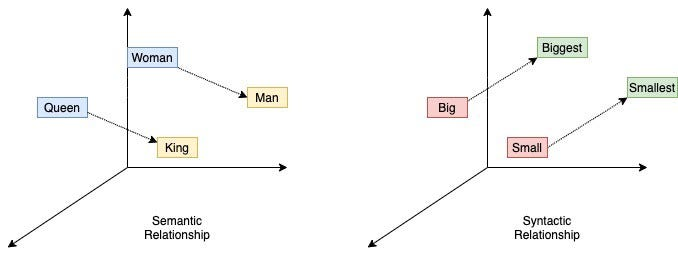
\includegraphics[width=\textwidth,height=0.8\textheight,keepaspectratio]{images/vector-space/glove-2.png}
        \caption*{\tiny Source: N. Birajdar, ``Word2Vec Research Paper Explained'', Towards Data Science, 16 March 2021 (figure by the author).}
    \end{figure}
\framebreak
    \begin{figure}
        \centering
        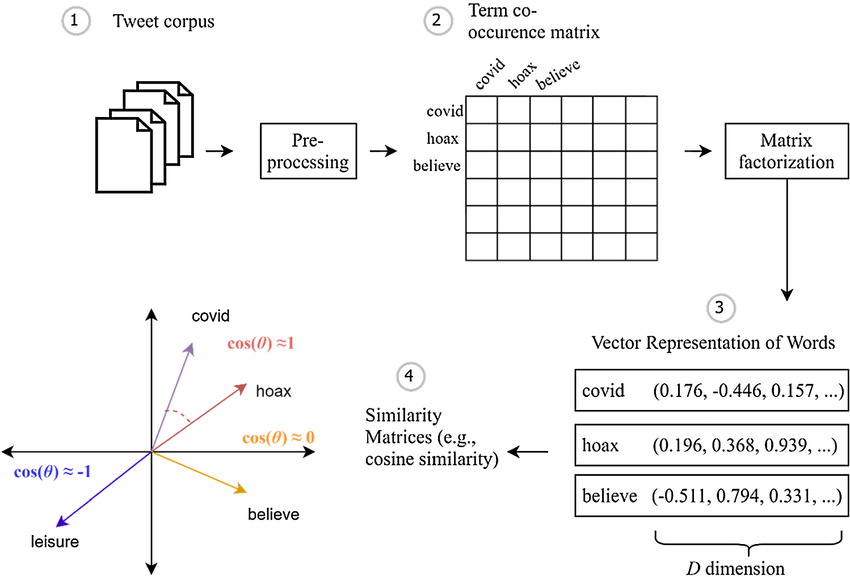
\includegraphics[width=\textwidth,height=0.8\textheight,keepaspectratio]{images/vector-space/glove-1.png}
        \caption*{\tiny Source: Batzdorfer et al., ``Conspiracy theories on Twitter: emerging motifs and temporal dynamics during the COVID-19 pandemic'', \textit{International Journal of Data Science and Analytics} 13(4), 2022, Fig.~1 (CC BY 4.0).}
    \end{figure}
\end{frame}